\documentclass{article}
\usepackage[utf8]{inputenc}
\usepackage[letterpaper,total={5.5in,9in}, top=1.0in, inner=1.5in, outer=1.0in,bottom=1.0in,,headheight=0pt,headsep=0pt,centering]{geometry}
\title{Effect of different population of flower on the gland area, with the gland-stigma distance as the associated factor  }
\author{Pham Xuan Huy Nguyen}
\date{December 2022}
\usepackage{listings}
\usepackage{graphicx}
\begin{document}

\maketitle

\section{Background}

Reproduction is one of the most important part in a life cycle of a plant, and the phenotypes of flower in floral plants to attract pollinator of plants are what evolutionary botanists are interested in. The combination of different patterns among floral parts can affect the pollination process of pollinators. 9 populations of flowers in Costa Rica are selected and 9 measurements of floral part are made. In this research, we will investigate the effect of different population of flower on the gland area (GA), with the gland-stigma distance (GSD) as the associated factor. The GSD tells which size of pollinator will fit with the flower, while GA refers to the reward for the pollinator.

\section{Methods and Results}
\textbf{Homogeneity of regression slopes\\}

The following lines read the file data and plot the homogeneity of regression slopes.
In Figure 1, each colours represents the data from a particular measurement in GA and GSD, and the colours tell us the population. The lines are the regression slopes for the particular population. There are unequal positive relationships between GA and GSD in all populations except S20, which appears to be no relationship at all, giving doubt whether there is homogeneity of regression slopes. Many points fall outside the grey area, which indicate that the homogeneity may be violated.\\
\begin{lstlisting}[language=R]
blossoms = read.csv('blossoms.csv')
library(ggplot2)
ggplot(blossoms, aes(GSD,GA, colour=pop)) + 
geom_point() + stat_smooth(method=lm) + 
labs(title='Scatter plot of GA and GSD from different populations ',
x="Gland-stigma Distance(mm)",y="Gland Area(mm^2)")
\end{lstlisting}
\begin{figure}
    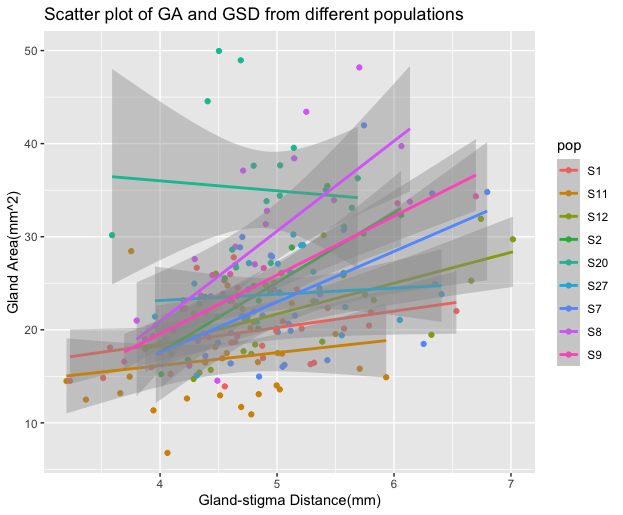
\includegraphics[width=\linewidth]{scatterplot.png}
    \caption{Display the relationship between GA and GSD for 9 populations (different colours).}
    \label{fig:my_label}
\end{figure}\break
\textbf{ANCOVA\\}

The following lines show the ANCOVA results of GA in different population with GSD as predictor and the interaction of population and GSD. \\
\begin{lstlisting}[language=R]
library(car)
md = aov(GA ~ GSD + pop + pop:GSD,data=blossoms)
Anova(md, type='III')
\end{lstlisting}
\lstinputlisting{md.txt}

The interaction between GSD and population is statistical significant, thus the homogeneity of regression slope is violated. We will proceed assuming the homogeneity of regression slopes assumption is violated. Next, we would like to check for independence of the covariant GSD and the treatment group population.\\

\begin{lstlisting}[language=R]
newmd = aov(GSD~pop, data=blossoms)

summary(newmd)
\end{lstlisting}
\lstinputlisting{indep.txt}

The model has statistical significant, we will proceed with assumption that we violate the independence assumption between the covariant and the treatment group.\\
\break
\textbf{Examine GA over different population when controlling for the GSD\\}
\begin{lstlisting}[language=R]
mdl = lm(GA ~ GSD + pop, data=blossoms)
anova(mdl)
\end{lstlisting}
\lstinputlisting{ancova2.txt}
\break
\begin{lstlisting}[language=R]
summary(mdl)
\end{lstlisting}

\lstinputlisting{ancova.txt}
Population S1 has smaller gland area than population S11 on average, and bigger gland area than any other population. From the R-square value, we can conclude this model explain 54.4\% of the variance in gland area.

\section{Conclusions}
There is not enough evidence to show that there is an interaction of population on the gland area with the gland-stigma distance as the associated factor.


\end{document}